
\chapter{Introduction and Background} 
\thispagestyle{myheadings} 
In this chapter, we first discuss regular types of sensors used for guarding or surveilence, 
with a focus on the line-based and range-based sensors. 
% and we then introduce the two types of simplified sensing model studied in this thesis, 
Then, a literature study on the related work of sensor placement and 
coverage-related geometric problems will be given. 
\section{Sensors Systems} 
Sensor systems are ubiquitous. To list a few, systems of radar antennas 
or other sensor sources are frequently used as base stations for signal transmission, 
defense system.
% Surveilence or tracking cameras surveillance and tracking system, 
Sensors like laser beams or cameras are usually used for indoor surveilence system or tracking system.

On top of autonomous vehicles, sensor system is indispensible 
e.g., Tesla used 12 ultrasonic sensors
near the front and rear bumper \footnote{https://www.tesla.com/en\_eu/support/transitioning-tesla-vision} 
and later changed into the camera vision system. 
TuSimple, a truck company, employs a combination of cameras, radars and lidars
for their perception system \footnote{https://www.tusimple.com/blogs/tusimple-1000-meter-perception-system}.

\begin{figure}[ht] 
    \centering 
    \begin{subfigure}[b]{0.32\textwidth} 
        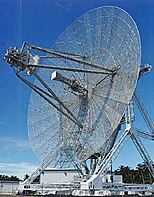
\includegraphics[width=\textwidth]{figures/Radar_antenna.jpg} 
        \caption{Radar antenna} 
        \label{fig:intro_radar} 
    \end{subfigure} 
    \begin{subfigure}[b]{0.55\textwidth} 
        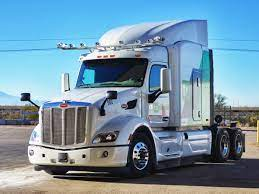
\includegraphics[width=\textwidth]{figures/truck_cam.jpeg} 
        \caption{Autonomous truck camera system} 
        \label{fig:intro_truckcam} 
    \end{subfigure} 
    \begin{subfigure}[b]{0.41\textwidth} 
        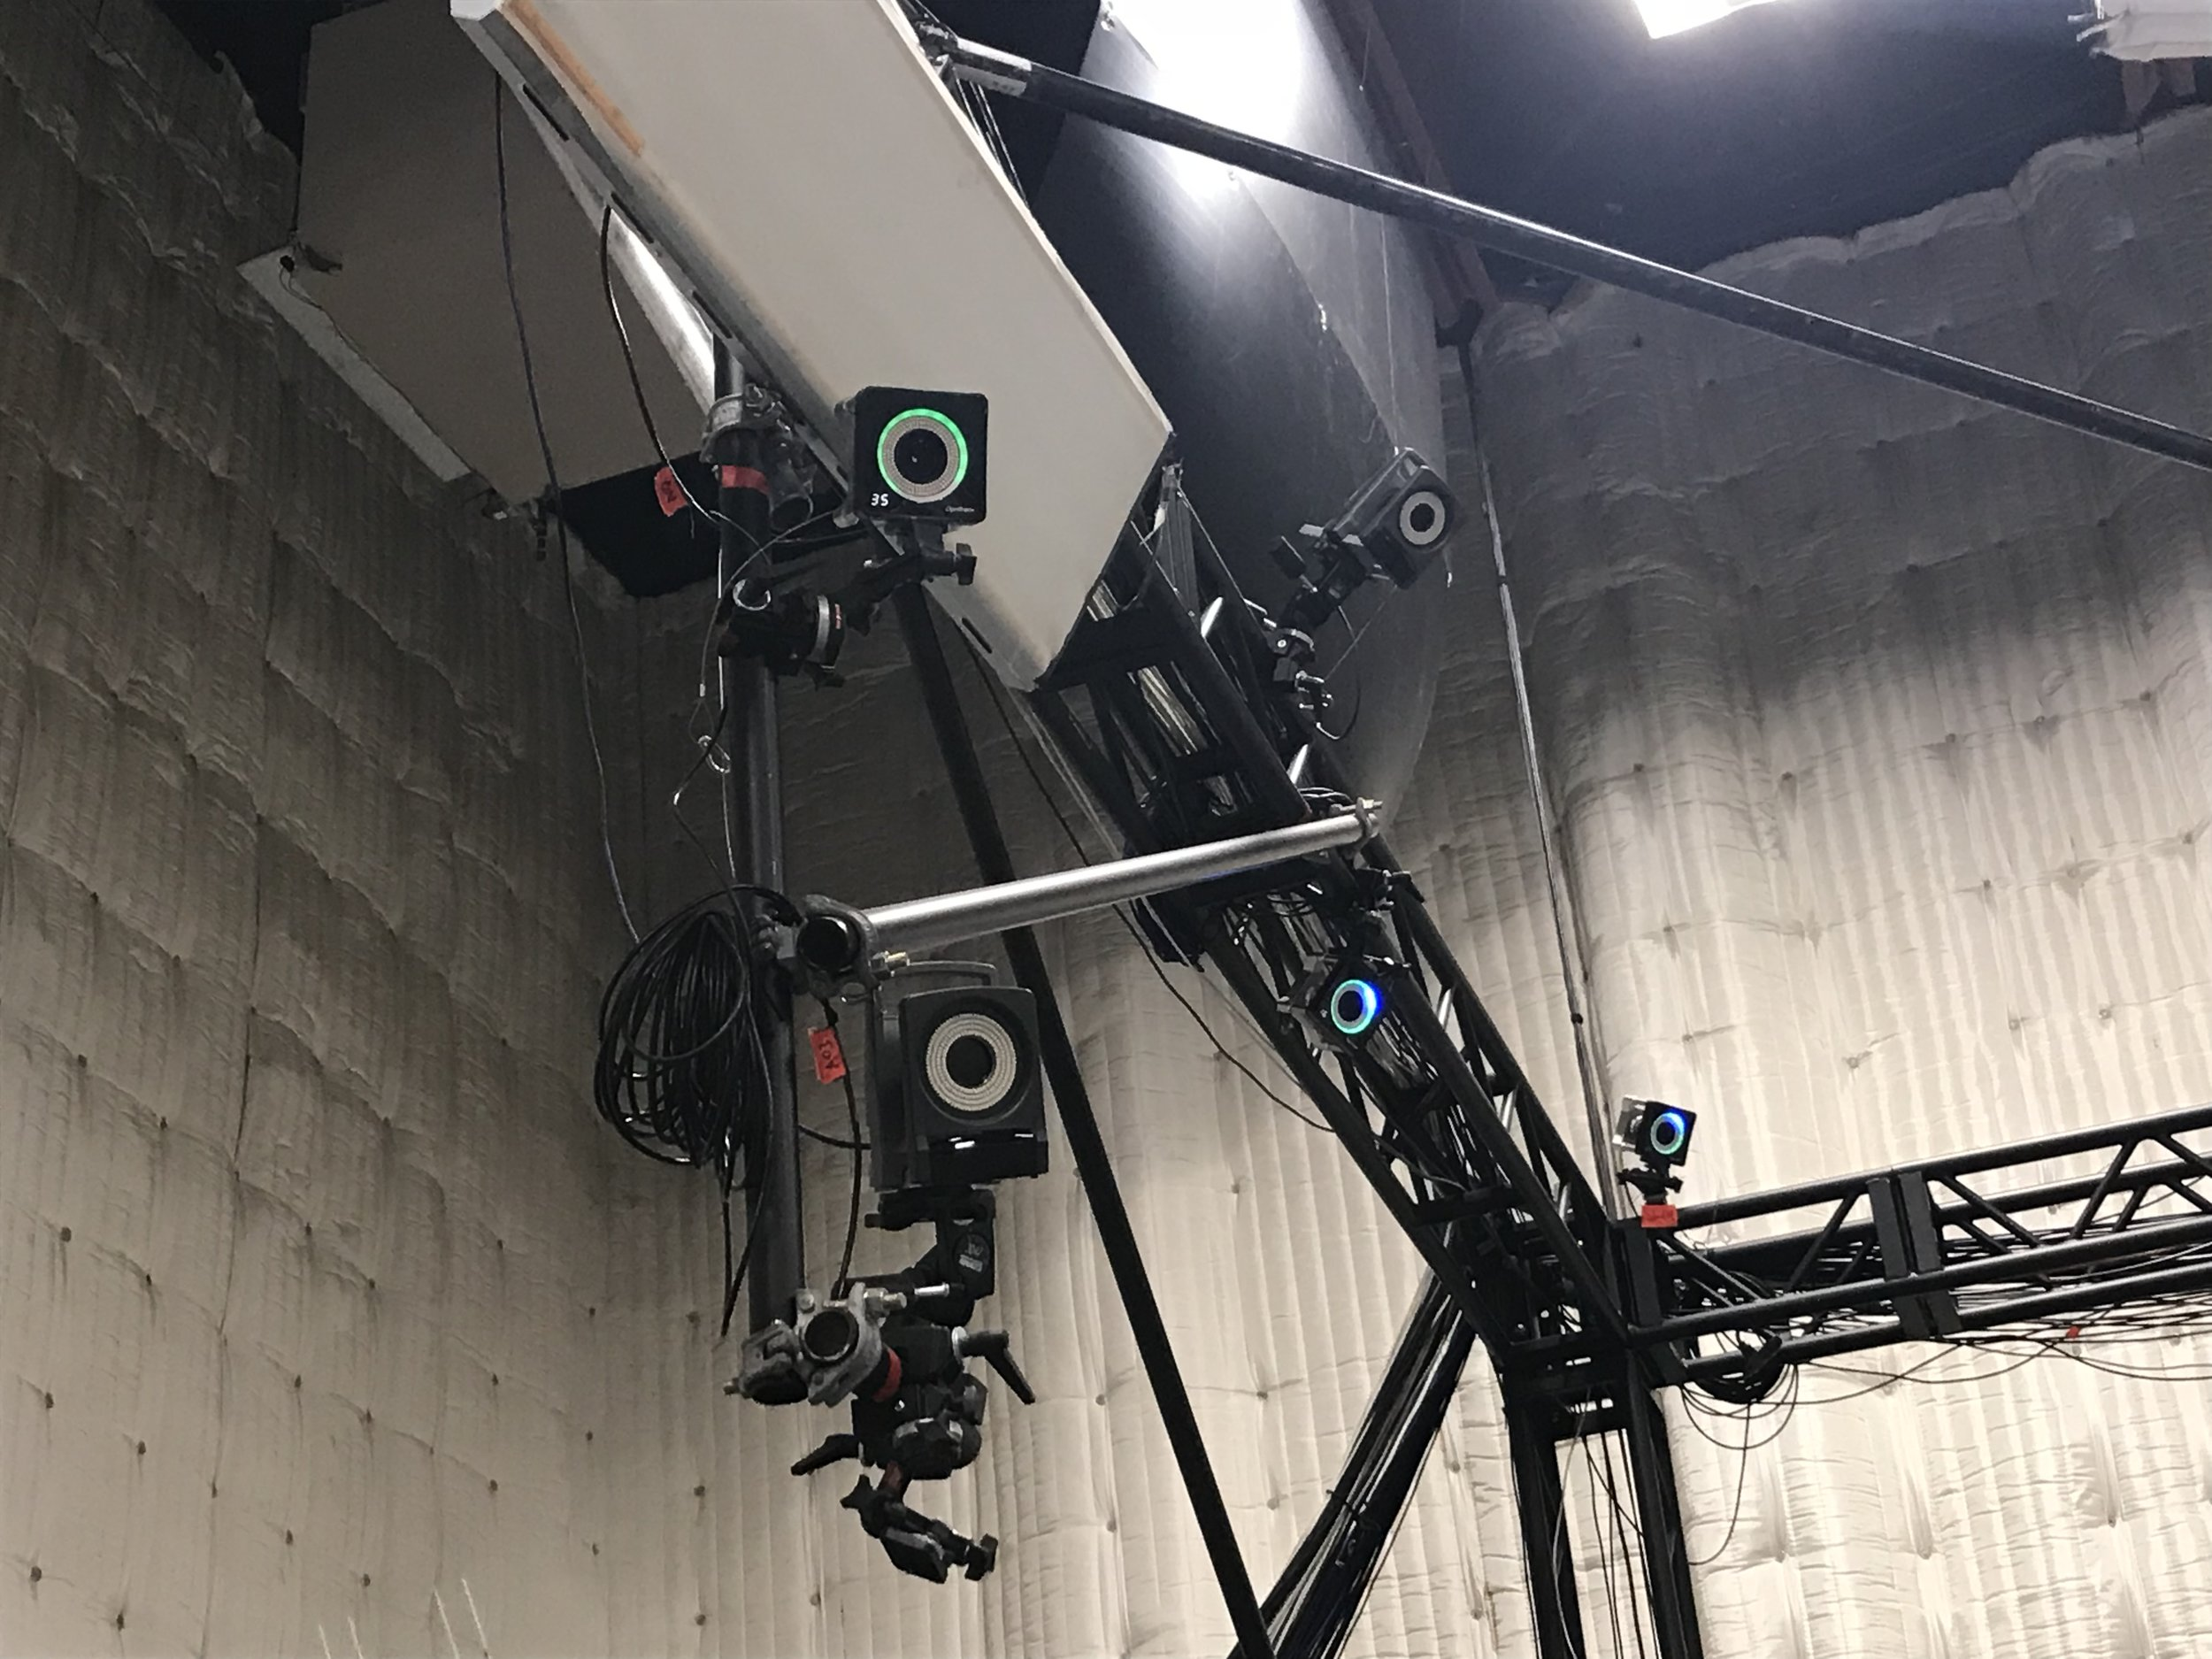
\includegraphics[width=\textwidth]{figures/optitrack.jpg} 
        \caption{Optical tracking system} 
        \label{fig:intro_optitrack} 
    \end{subfigure} 
    \begin{subfigure} [b]{0.46\textwidth} 
        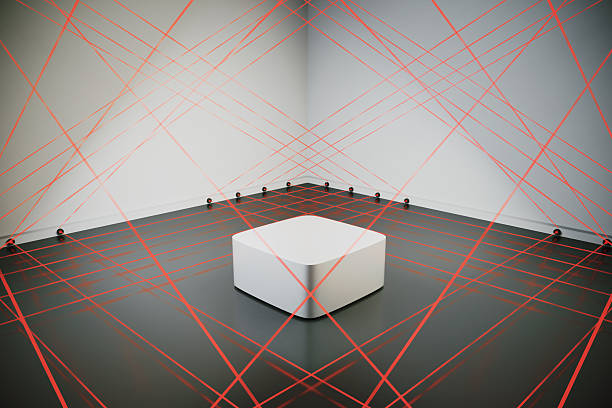
\includegraphics[width=\textwidth]{figures/laser.jpg} 
        \caption{Laser system} 
        \label{fig:intro_laser} 
    \end{subfigure} 
\end{figure} 

\section{Background}
\subsection{NP-hardness}
\subsection{Integer Programming}
\subsection{}
\section{Literature Seview} 
\subsection{Coverage-related problems in computational geometry} 

\subsection{Sensor network} 

\subsection{}
